
\documentclass[18pt, aspectratio=169]{beamer}
% \documentclass{etp-beamer-fancy}
\usepackage[utf8]{inputenc}
% \usepackage{templates/mytemplate}
\usepackage{templates/beamerthemekit}
\usepackage{graphicx}
\usepackage{microtype}
\usepackage{xcolor}
\usepackage{hyperref}
\usepackage{siunitx}
\usepackage{upgreek}
\usepackage{hepnames}
\usepackage{appendixnumberbeamer}
\usepackage{booktabs}
\NewDocumentCommand\angrange{O{} m m}{\SIrange[parse-numbers=false,#1]{\ang[parse-numbers=true]{#2}}{\ang[parse-numbers=true]{#3}}{}}
\usepackage{subcaption}
% \usepackage{enumitem}

\title{Track Quality Estimator -- Kinematic Distributions}
\subtitle{Tracking Meeting}
\author[Michael Eliachevitch
(\href{mailto:michael.eliachevitch@kit.edu}{michael.eliachevitch@kit.edu})]{Michael Eliachevitch(\href{mailto:michael.eliachevitch@kit.edu}{michael.eliachevitch@kit.edu})}
\titleimage{tracks_wide}
\titlelogo{belle2-logo}
\institute[ETP -- KIT]{Institut für Experimentelle Teilchenphysik (ETP) -- KIT}
\date{10 Mai 2019}

\newcommand{\kitemph}[1]{\textcolor{kit-green100}{\bf{#1}}}

\begin{document}
\maketitle

\begin{frame}
  \frametitle{Reminder:  MVA Track Quality Estimator peformance}
  \begin{columns}
    \begin{column}{.33\textwidth}
      \centering
      \includegraphics[width=\textwidth]{figures/combined-qi/fullqi_findeff.pdf}\\
    \end{column}
    \begin{column}{.33\textwidth}
      \centering
      \includegraphics[width=\textwidth]{figures/combined-qi/fullqi_fake_rate.pdf}\\
    \end{column}
    \begin{column}{.33\textwidth}
      \centering
      \includegraphics[width=\textwidth]{figures/combined-qi/fullqi_clone_rate.pdf}
    \end{column}
  \end{columns}
  \begin{columns}
    \begin{column}{.4\textwidth}
      \centering
      ROC
      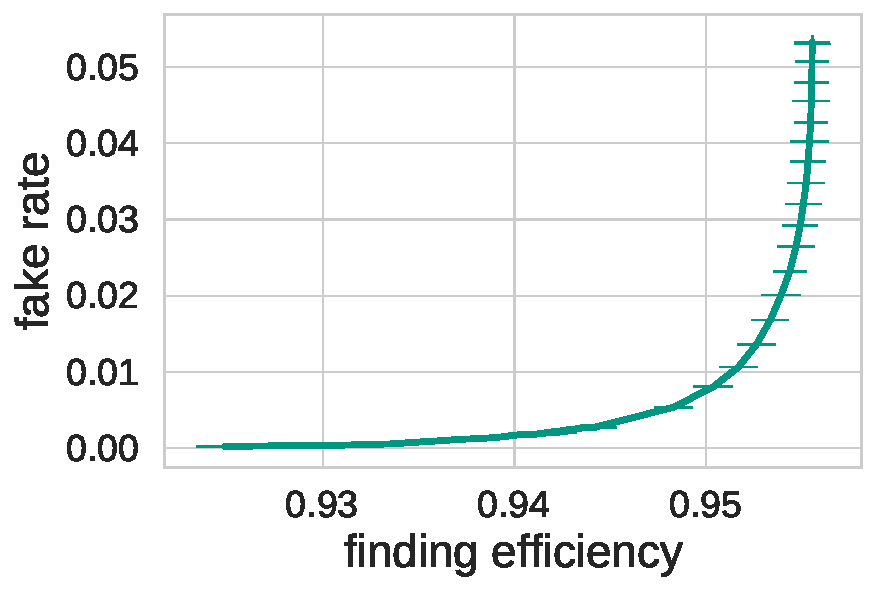
\includegraphics[width=\textwidth]{figures/combined-qi/fullqi_roc_curve.pdf}
    \end{column}
    \begin{column}{.6\textwidth}
      \begin{block}{Goal of this study}
    See in which kinematic region, i.e.\ for which track parameters, tracks get bad quality
    indicators assigned and get thus rejected when cutting on it.
  \end{block}
    \end{column}
  \end{columns}
\end{frame}

\begin{frame}
  \frametitle{Track parameter distributions}
  \begin{columns}
    \begin{column}{.5\textwidth}
      \centering
      \includegraphics[width=.9\textwidth]{figures/combined-qi/pt_distributions_by_qi.pdf}
      \includegraphics[width=.9\textwidth]{figures/combined-qi/phi0_distributions_by_qi.pdf}
    \end{column}
    \begin{column}{.5\textwidth}
      \centering
      \includegraphics[width=.9\textwidth]{figures/combined-qi/d0_distributions_by_qi.pdf}
      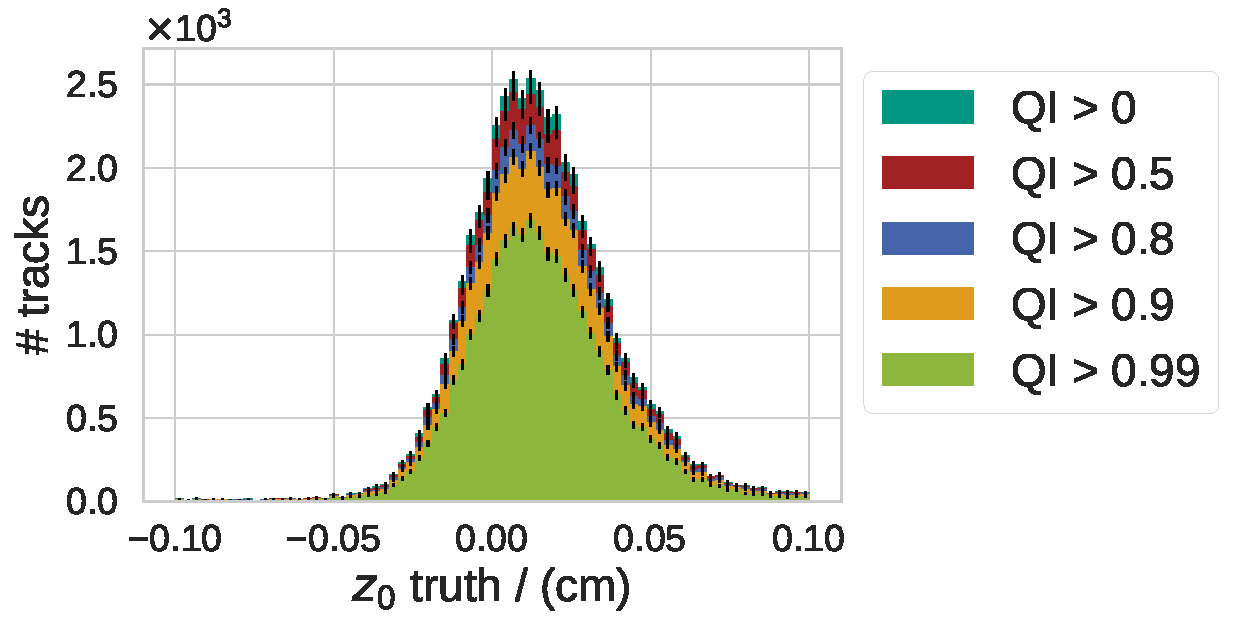
\includegraphics[width=.9\textwidth]{figures/combined-qi/z0_distributions_by_qi.pdf}
    \end{column}
  \end{columns}
  \begin{itemize}
  \item plotted are matched and clone tracks
  \end{itemize}
\end{frame}

\begin{frame}
    % \frametitle{$\tan{\lambda}$: Peak with bad quality indicator tracks at 0?}
  \begin{columns}
    \begin{column}{.5\textwidth}
      \centering
      \includegraphics[width=.9\textwidth]{figures/combined-qi/tan_lambda_distributions_by_qi.pdf}      
    \end{column}
    \begin{column}{.5\textwidth}
      \centering
      \includegraphics[width=.9\textwidth]{figures/combined-qi/nhits_distributions_by_qi.pdf}      
    \end{column}
  \end{columns}
  \begin{itemize}
  \item peak at $\tan{\lambda} = 0$ from clones
  \end{itemize}
\end{frame}

\begin{frame}
  \frametitle{$\tan{\lambda}$ stacked distribution}
  \begin{center}
    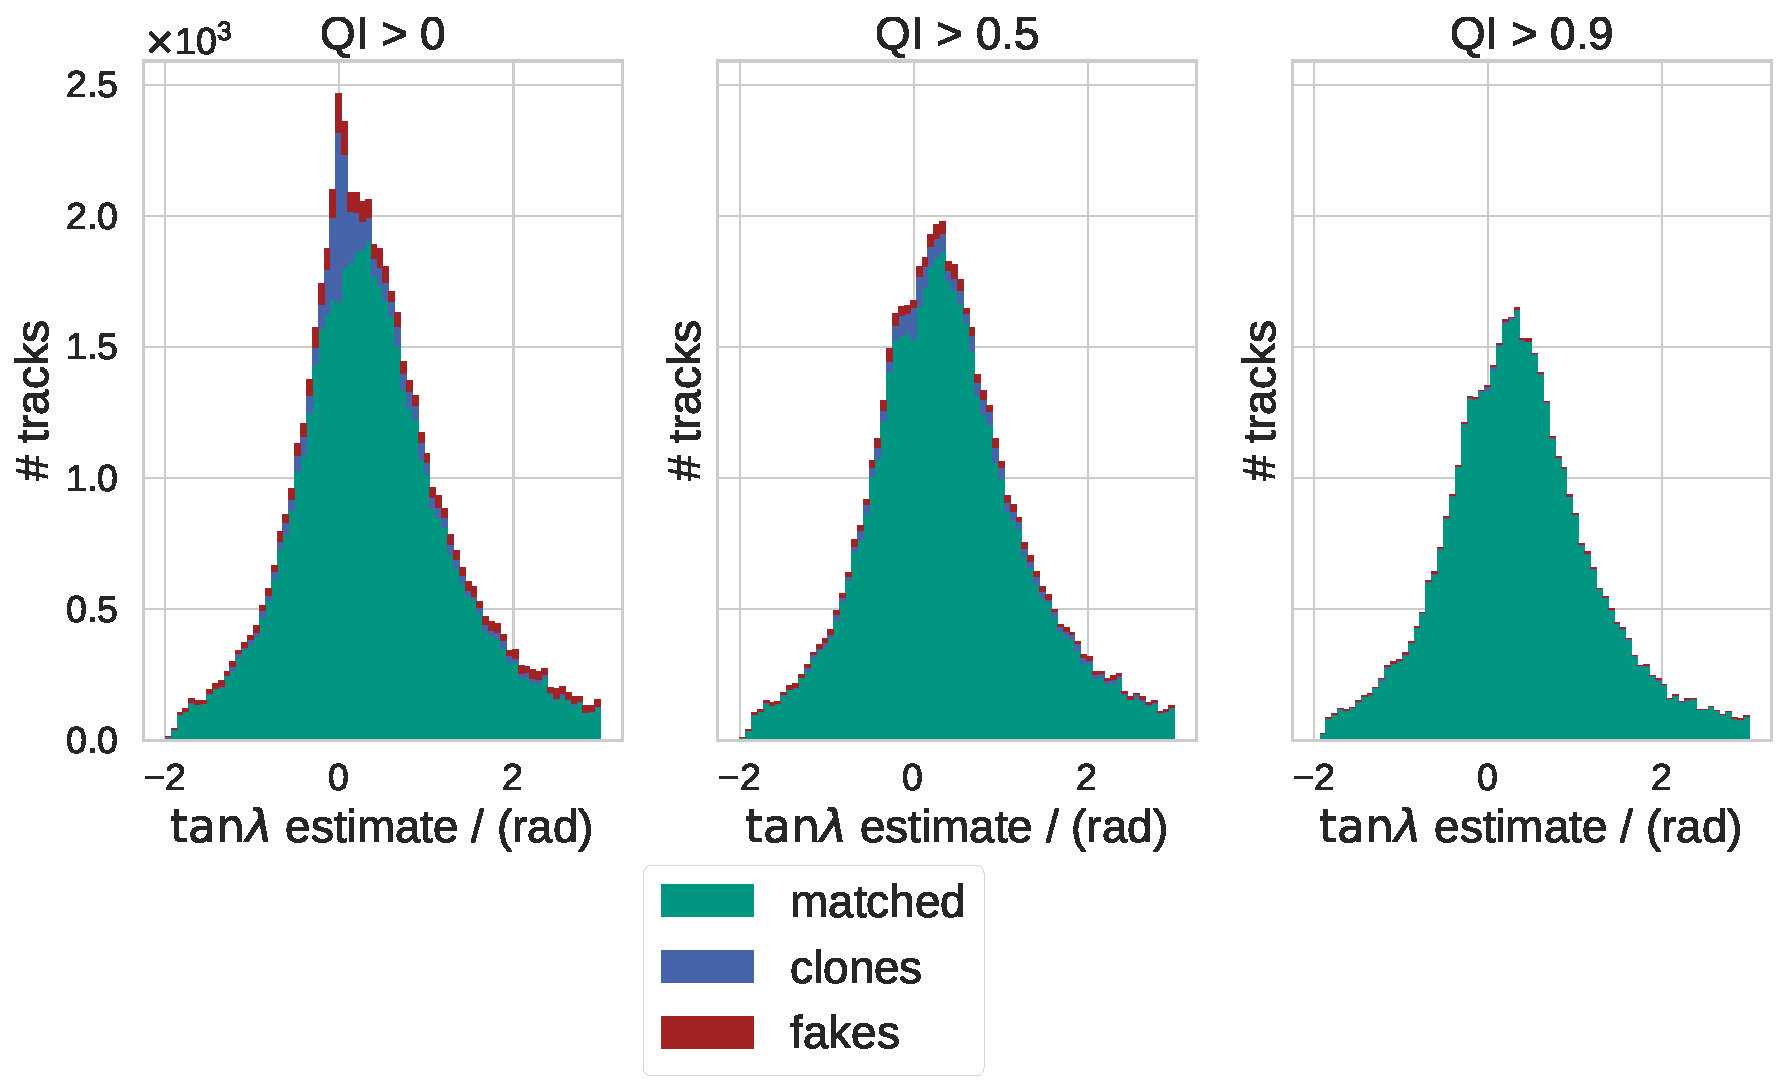
\includegraphics[width=.7\textwidth]{figures/combined-qi/tan_lambda_stacked_distributions_by_qi.pdf}
  \end{center}
\end{frame}

\begin{frame}
  \frametitle{$p_T$ stacked distribution}
  \begin{center}
    \includegraphics[width=.7\textwidth]{figures/combined-qi/pt_stacked_distributions_by_qi.pdf}
  \end{center}
\end{frame}

\begin{frame}
  \frametitle{nHits stacked distribution}
  \begin{center}
    \includegraphics[width=.7\textwidth]{figures/combined-qi/nhits_stacked_distributions_by_qi.pdf}
  \end{center}
\end{frame}

\end{document}

%%% Local Variables:
%%% coding: utf-8
%%% mode: LaTeX
%%% TeX-engine: default
%%% TeX-master: t
%%% fill-column: 100
%%% ispell-dictionary: "english"
%%% eval: (flyspell-mode 1)
%%% eval: (add-to-list 'TeX-outline-extra '("\\\\frametitle\\b" 7))
%%% End: